\scanpage{89}

\reversemarginpar
\margin{$\unsure{k}$\par
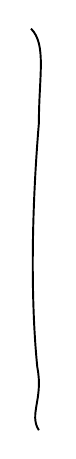
\begin{tikzpicture}[x=1mm,y=1mm,baseline=0pt]
\draw[line width=.7pt] (0,0) .. controls (2,-2) and (1,-6) .. (1,-12)
 .. controls (0,-24) and (0,-35) .. (.8,-43)
 .. controls (1.6,-47) and (-.3,-49) .. (1,-51);
\end{tikzpicture}}
\normalmarginpar

\[
\begin{array}{ll}
(18)&\displaystyle
\deleted{\unsure{f(\rho|f(\rho)}}
\sum_1^{\unsure{n|k}}f(|\lambda_i|)\leq\sum_1^k f(\rho_i)
\qquad
\overset{\inserted{(k:1,\ldots)}}{\deleted{(k\leq\dim\unsure{H|E})}}
\end{array}
\]

In particular, \deleted{\unsure{in order that}} if
\deleted{\unsure{$\dim$}}\inserted{$E$} is of infinite dimension,
if \inserted{the series} $\sum_{i=0}^{\infty}f(\rho_i)$
\deleted{\unsure{converges, then|converges, then|converges, then}}\inserted{is convergent},
the same holds for
$\sum_{\unsure{j|i}\unsure{\geq|=}0}^{\unsure{-\infty|\infty}}f(|\lambda_i|)$, and we have

\[
\begin{array}{ll}
(19)&\displaystyle\sum_{i=1}^{\infty}f(|\lambda_i|)\leq\sum_{i=0}^{\infty}f(\rho_i)
\end{array}
\]

In particular, taking $f(\unsure{a|r})=r^p$ $(p>0)$, we deriv\unsure{e}

\uline{Corollary 2} Let $u$ be a compact operator in a
\reversemarginpar
\margin{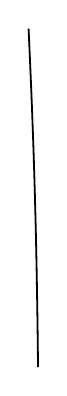
\begin{tikzpicture}[x=1mm,y=1mm,baseline=0pt]
\draw[line width=.65pt] (0,0) .. controls (.5,-11) and (1,-23) .. (1.2,-43);
\end{tikzpicture}}
\normalmarginpar
Hilbert space $E$, and let $p>0$. Then, for every integer $k>0$

\[
\begingroup
\setbox0=\hbox{$\displaystyle\sum_{i=1}^k|\lambda_i|^p\leq\sum_{\unsure{j|i}=1}^k\rho_i^p=$}
\setbox2=\hbox{$\displaystyle\deleted{\|u\|_p}$}
\begin{array}{ll}
(20)&
\smash{\rlap{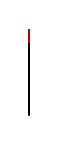
\begin{tikzpicture}[x=\wd0,y=1ex,baseline=0pt]
\draw[red!75!black,line width=1pt] (-.025,-3.2)--(-.02,3.4)--(1.09,3.9);
\draw[red!75!black,line width=1pt] (1.02,3.0)--(1.025,-3.15)--(-.025,-3.2);
\draw[red!75!black,line width=.8pt] (-.025,-3.35) .. controls (.35,-3.35) and (.8,-3.0) .. (1.025,-2.95);
\draw[line width=.6pt] (.025,2.7)--(-.07,1.6)--(.025,2.3)--(-.07,-.3)
 --(.04,.3)--(-.03,-3.3)--(.19,-1.75)--(.08,-3.3)--(.48,-1.5)
 --(.39,-3.2)--(.65,-1.4)--(.61,-2.7)
 .. controls (.79,-2.2) and (.93,-2.25) .. (.97,-2.5);
\end{tikzpicture}}}\box0\hspace{.5em}
\smash{\rlap{\begin{tikzpicture}[x=\wd2,y=1ex,baseline=0pt]
\draw[line width=.6pt] (-.1,3.5)--(1.14,3.4)--(1.18,-2.55);
\draw[line width=.6pt] (1.0,-2.5) .. controls (.5,-2.9) and (.05,-2.85) .. (-.2,-2.5);
\draw[line width=.7pt] (.1,3.45)--(-.22,1.7)--(.42,3.35)--(-.08,.8)--(.57,2.0)--(.1,-.1)--(.98,-.25);
\end{tikzpicture}}}\box2
\qquad
\setbox4=\hbox{$\deleted{(k\leq\dim\unsure{H|E})}$}
\smash{\rlap{\begin{tikzpicture}[x=\wd4,y=1ex,baseline=0pt]
\draw[line width=.6pt] (.01,1.85)--(.095,1.5)--(.205,2.7)--(.145,.95)--(.36,2.55)--(.28,.55)--(.55,1.95)--(.47,.5)--(.92,1.35);
\end{tikzpicture}}}\box4
\end{array}
\endgroup
\]

\deleted{\unsure{in particular}, if $E$ is of finite dimension $n$}

\[
\begingroup
\setbox0=\hbox{$\displaystyle\sum_i|\lambda_i|^p\leq\sum_i\rho_i^p=\|u\|_p$}
\begin{array}{ll}
(21)&\smash{\rlap{\begin{tikzpicture}[x=\wd0,y=1ex,baseline=0pt]
\draw[red!75!black,line width=1pt] (-.03,3.45)--(-.025,-2.9)
 .. controls (.4,-2.85) and (.8,-2.6) .. (1.035,-2.55);
\draw[red!75!black,line width=1pt] (1.055,2.6)--(1.05,-2.25);
\draw[red!75!black,line width=1pt] (-.02,3.55) .. controls (.4,3.8) and (.75,3.8) .. (1.07,3.5);
\end{tikzpicture}}}\box0
\end{array}
\endgroup
\]

(where the sum is taken over all indices $i$) In particular, taking $p=1$ and $p=2$,
and \unsure{applying|using} number 1, theorem 2 and theorem 3, formulas (15) and (20), we find

\uline{Corollary 3} Let $u$ be a Fredholm operator \deleted{\unsure{whose}}
(respectively an \deleted{\unsure{Hilb|Hilb.}} H.-S. operator) in
\deleted{the \unsure{space|area}}\inserted{a space} of Hilbert.
\deleted{\unsure{And,|And}} Then \deleted{\unsure{a}} the sequence of eigenvalues
is summable (respectively square-summable) and we have

\[
\begingroup
\setbox0=\hbox{$\displaystyle\sum|\lambda_i|\leq\|u\|_1$}
\setbox2=\hbox{$\displaystyle\left(\sum|\lambda_i|^2\right)^{1/2}\leq\|u\|_2$}
\begin{array}{ll}
(21)&\smash{\rlap{\begin{tikzpicture}[x=\wd2,y=1ex,baseline=0pt]
\draw[red!75!black,line width=1pt] (-.03,2.8)--(-.05,-1.8)--(.98,-1.7)--(.995,2.55);
\draw[red!75!black,line width=1pt] (.1,3.0) .. controls (.4,3.3) and (.7,3.2) .. (1.07,2.95);
\end{tikzpicture}}}\hbox to\wd2{\box0\hfil}\\[2.7ex]
(22)&\smash{\rlap{\begin{tikzpicture}[x=\wd2,y=1ex,baseline=0pt]
\draw[red!75!black,line width=1pt] (-.05,3.4) .. controls (.25,3.25) and (.75,3.6) .. (1.03,3.45);
\draw[red!75!black,line width=1pt] (-.065,2.8)--(-.065,-2.45)
 .. controls (-.06,-2.85) and (-.04,-2.95) .. (0,-2.9)--(1.04,-2.55);
\draw[red!75!black,line width=1pt] (1.055,2.8)--(1.07,-2.7);
\end{tikzpicture}}}\box2
\end{array}
\endgroup
\]

Let us also mention the

\uline{Corollary 4} Let $u$ be a \inserted{linear} operator \deleted{\unsure{in}} in a
\reversemarginpar
\margin{\shortstack[l]{small\\type}\par
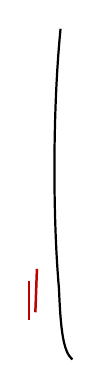
\begin{tikzpicture}[x=1mm,y=1mm,baseline=0pt]
\draw[line width=.8pt] (1,0) .. controls (0,-10) and (0,-24) .. (.8,-33)
 .. controls (1,-38) and (1.3,-41) .. (2.5,-42);
\draw[red!75!black,line width=1pt] (-3,-32)--(-3,-37);
\draw[red!75!black,line width=.9pt] (-2,-30.5)--(-2.2,-36);
\end{tikzpicture}}
\normalmarginpar
Hilbert space of finite dimension $n$, \deleted{Then,} let
$f(s_1,\mathord{-}s_n)$ \deleted{\unsure{is}} be a function of \inserted{$n$} arguments $s_i>0$
such that $f(e^{t_1},\mathord{-}e^{t_n})$ is convex (not necessarily increasing).
If $f$ is in fact defined and continuous for \deleted{\unsure{the}} $s_i\geq0$,
or if $u$ is invertible, we have

\[
\begingroup
\setbox0=\hbox{$\displaystyle f(|\lambda_1|,\mathord{-}|\lambda_n|)\leq f(\rho_1,\mathord{-},\rho_n)$}
\begin{array}{ll}
\text{\textcircled{23}}&
\smash{\rlap{\begin{tikzpicture}[x=\wd0,y=1ex,baseline=0pt]
\draw[line width=.65pt] (.13,3.45) .. controls (.4,3.1) and (.75,3.6) .. (1.02,3.55);
\draw[line width=.75pt] (-.025,2.85)--(-.025,-1.55)
 .. controls (-.02,-2.1) and (.02,-2.25) .. (.08,-2.15)
 .. controls (.42,-1.7) and (.78,-1.75) .. (1.015,-1.75);
\end{tikzpicture}}}\box0\unsure{!|.}
\end{array}
\endgroup
\]

\deleted{\unsure{(23)|Then}} Indeed, we have, in addition to the inequalities
$|\lambda_1\mathord{-}\lambda_n|\leq\rho_1\mathord{-}\rho_n$ $(k\leq n)$, the \uline{equality}

\reversemarginpar\margin{90}\normalmarginpar
